\documentclass{ctexart}
\usepackage{amsmath}
\usepackage{graphicx}
\usepackage{esint}
\usepackage{float}
\usepackage{ulem}
\usepackage{geometry}
\setCJKmainfont{HarmonyOS Sans SC}
\geometry{a5paper,left=2cm,right=2cm,top=1cm,bottom=1cm}
\pagestyle{empty}
\author{九鸟}
\title{大雾二寄结论速寄v1.1}
\date{}
\def\ooint{{\bigcirc}\kern-12.5pt{\int}\kern-7.5pt{\int}}
\begin{document}
\maketitle
\section{序 - 食用指难}
这是一份总结二级结论以及一些难记的概念的笔记,
主要是为了方便复习,所以几乎无推导,
只会有一些重要的结论和一些重要的公式。
当然在源文件里面保留了一点过程,
如有需要自行取消注释进行编译或找我要。
当然中间也有一丁点的私货题目来解释自己的私货结论。
要是有错误的话欢迎指正。
但本人对于这份笔记的正确性不会负任何的责任,
以及其中出现不能保证是考点,
如果因为笔记的错误记错了什么丢分的话,
找阿giao会帮你补的。
莲祝你食用愉快。项目已经开源,地址:https://github.com/RastyASWoz/PhyXA.git


v1.1修正内容:修复了部分的typo。鸣谢@alphabet 找出的typo,鸣谢@Zjl37 提供的排版建议。
\begin{figure}[H]
    \centering
    
\includegraphics[width=0.5\textwidth]{img/lian.jpg}
    \caption[ ]{只要你也喜欢莲那我们就是\sout{情敌}朋友了}
\end{figure}
\section{第二章}
\subsection{“欧拉公式”}
\begin{figure}[H]
    \centering
    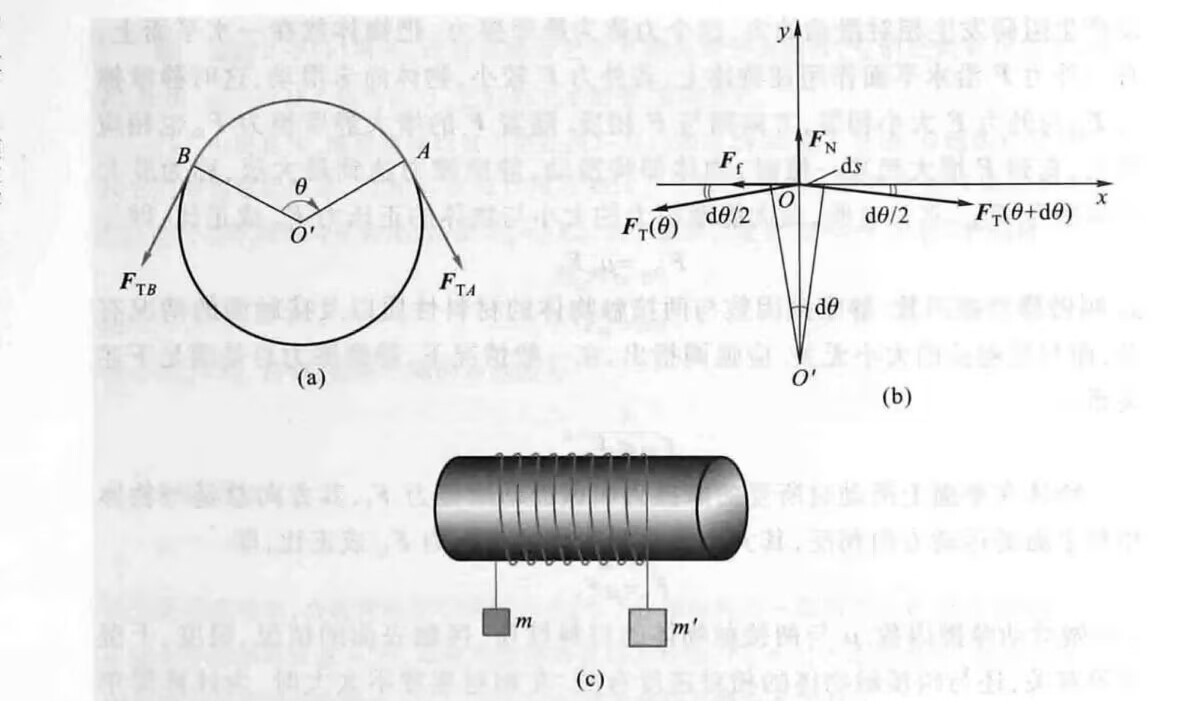
\includegraphics[width=0.7\textwidth]{img/ola.jpg}
\end{figure}
将绳子绕在一个固定的轴上,
给其一端$F_1$的力,
若想在另一端施加一个$F_2$的力想使得绳子与轴发生滑动,
则
$$
    F_{2min} = F_1 e^{\mu \theta}
$$
% \begin{align*}
%     F(\theta)' &= \mu F(\theta) \\
%     \Rightarrow F(\theta) &= F(0) e^{\mu \theta}
% \end{align*}
\subsection{圆周运动}
在圆周运动中,有:
\begin{align*}
    \vec{a} &= \vec{\alpha} \times \vec{r} + \vec{\omega} \times \vec{v} \\
\end{align*}
对于匀变速圆周运动,类比直线运动,有:
\begin{align*}
    \theta &= \theta_0 + \omega_0 t + \frac{1}{2} \alpha t^2 \\
    \omega &= \omega_0 + \alpha t \\
    2 \alpha \theta &= \omega^2 - \omega_0^2 \\
\end{align*}
\section{第三章}
\subsection{质量相等的物体的弹性碰撞}
当两物体发生正碰时,有:
\begin{align*}
    \begin{cases}
        \vec{v_1'} = \vec{v_2} \\
        \vec{v_2'} = \vec{v_1}
    \end{cases}
\end{align*}
当两物体发生斜碰时(这里指一个动物体去碰撞另一个静止的物体),有:
$$
    \vec{v_1'} \perp \vec{v_2}
$$
% 斜碰情况的证明:\\
% 由柯尼希定理,对于一个二质点的系统有:
% $$
%     \frac{1}{2}m_1v_1^2 + \frac{1}{2}m_2v_2^2 =
%     \frac{1}{2}(m_1 + m_2)\left(\frac{m_1 \vec{v_1} +m_2 \vec{v_2} }{m_1 +m_2}\right)^2
%     + \frac{1}{2}\frac{m_1 m_2}{m_1 + m_2}(\vec{v_1} - \vec{v_2})^2
% $$
% 那么显然,在斜碰的情况下也是成立的。\\
% 那么由动能守恒和动量守恒,对照上式中的各项可以得到:
% \begin{align*}
%     \begin{cases}
%         \vec{v_1'} + \vec{v_2'} = \vec{v} \\
%         \vert \vec{v_1'} - \vec{v_2'} \vert = \vert \vec{v} \vert
%     \end{cases}
% \end{align*}
% 那么易知$\vec{v_1'} \perp \vec{v_2}$,据此求出$\vec{v_1'}$和$\vec{v_2'}$就不难了。
\subsection{质量不等的物体的弹性碰撞}
由动量守恒和动能守恒,可以得到:
\begin{align*}
    \begin{cases}
        m_1v_1' + m_2v_2' = m_1v_1 + m_2v_2 \\
        v_1' - v_2' = v_2 - v_1
    \end{cases}
\end{align*}
\footnote{请注意这里的方向,我们其实知道,对于上面的方程,一定是两个解,那么易知,$ |v_1 - v_2| $对应的两个解是方向相反的}
接下来可得:
\begin{align*}
    \begin{cases}
        v_1' = \frac{m_1 - m_2}{m_1 + m_2}v_1 + \frac{2m_2}{m_1 + m_2}v_2 \\
        v_2' = \frac{2m_1}{m_1 + m_2}v_1 + \frac{m_2 - m_1}{m_1 + m_2}v_2
    \end{cases}
\end{align*}
如果记忆不住,可以考虑记忆上上面的式子,然后用行列式进行推导。\footnote{这个行列式非常简单,现推完全来得及}
\subsection{系统内的质量转移}
\begin{figure}[H]
    \centering
    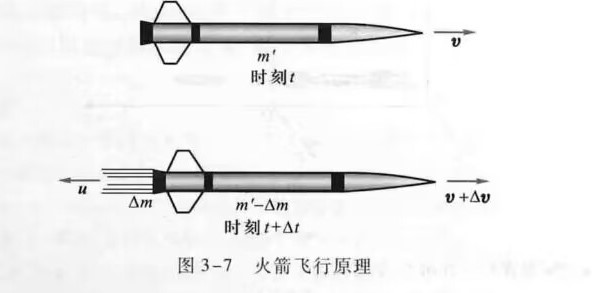
\includegraphics[width=0.5\textwidth]{img/3-7.jpg}
\end{figure}
当火箭系统受到的外力为$F$时,喷出气体的速度为$u$时有:
$$
    m(t) v'(t) = F + u m'(t)
$$
解得:
$$
    v(t) = v_0 + \int_0^t \frac{F}{m(t)}dt + u \ln \frac{m_0}{m(t)}
$$
特别的,如果$F = 0$,那么有:
$$
    v(t) = v_0 + u \ln \frac{m_0}{m(t)}
$$
当最后火箭燃烧后的质量为$m'$时,那么火箭的最终速度为:
$$
    v = v_0 + u \ln \frac{m_0}{m'}
$$
其中$\frac{m_0}{m'}$被称为质量比N,而这便是齐奥尔科夫斯基公式。
\section{第四章}
\subsection{转动惯量与力矩与角动量}
对于一个质点系,其转动惯量为:
$$
    J = \iint_{D} \rho \vec{r}^2 d \sigma
$$
一个力的力矩为:
$$
    M = \vec{r} \times \vec{F}
$$
转动定理表述为:
$$
    M = J \alpha
$$
角动量为:
$$
    \vec{L} = m \vec{r} \times \vec{v} = J \vec{\omega}
$$
有:
$$
    \vec{M} = \frac{d\vec{L}}{dt}
$$
故可以类比冲量定理使用冲量矩定理:
$$
    \Delta \vec{L} =J_2\omega_2 - J_1\omega_1 = \int_{t_1}^{t_2} \vec{M} dt
$$
式子的后半部分更具有普适性,故更常用。\\
力矩做功的公式为:
$$
    W = \int_{\theta_1}^{\theta_2} M d\theta
$$
力矩的功率为:
$$
    P = \vec{M} \cdot \vec{\omega}
$$
刚体的转动动能为:
$$
    T = \frac{1}{2} J \omega^2
$$
\subsection{各种形状的物体的转动惯量}
\begin{figure}[H]
    \centering
    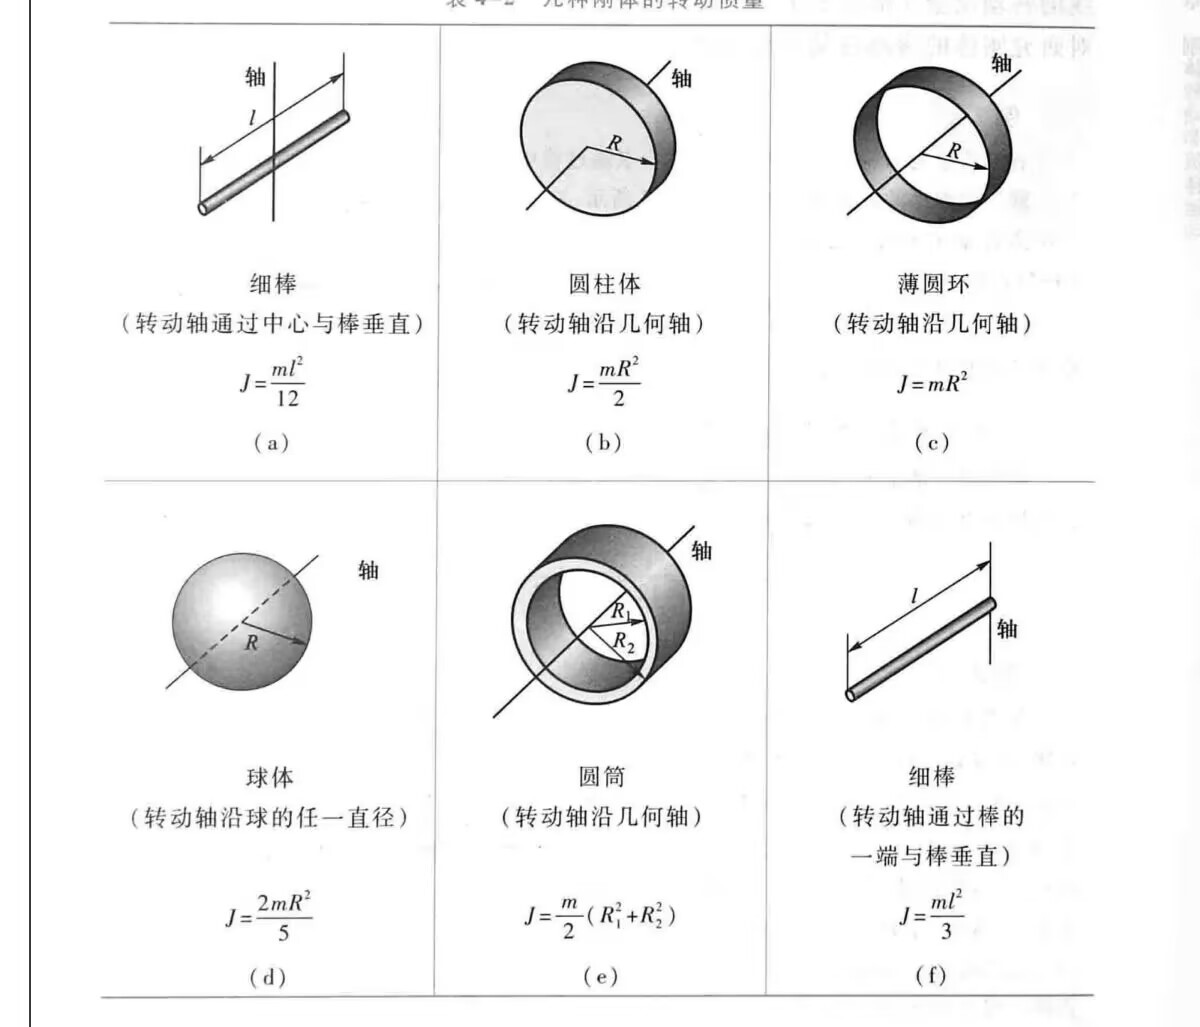
\includegraphics[width=0.9\textwidth]{img/4-2.jpg}
\end{figure}
\subsection{滑轮的等效质量}
\begin{figure}[H]
    \centering
    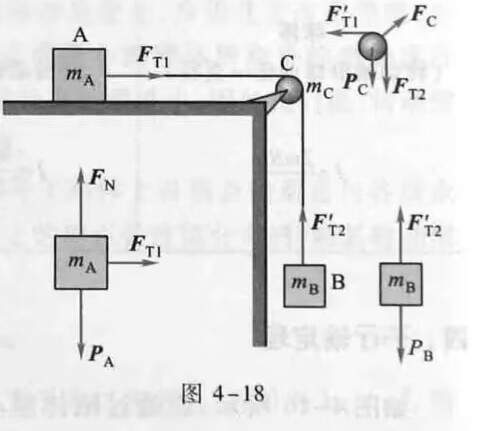
\includegraphics[width=0.5\textwidth]{img/4-18.jpg}
\end{figure}
对于如图所示的滑轮,
当其上面的绳子没有发生相对滑动的时候,
可以认为绳子连接了一个质量为$\frac{m_c}{2}$的物体。
证明:\\
\begin{align*}
    J       & = \frac{1}{2}m_c r^2                  \\
    M       & = (F_A - F_B)r                        \\
    M       & = J \alpha                            \\
    a       & = \alpha r                            \\
    m_{eq}  & = \frac{F_A - F_B}{a} = \frac{J}{R^2} \\
            & = \frac{m_c}{2}
\end{align*}
\subsection{转动惯量的平行轴定理}
设通过质心的轴的转动惯量为$J_0$,质心到平行轴的距离为$d$,则有:
$$
    J = J_0 + md^2
$$
证明:\\
\begin{align*}
    J_0 & = \iint_{D} \rho \vec{r}^2 d \sigma                                                                                                                   \\
    J   & = \iint_{D} \rho (\vec{r} + \vec{d})^2 d \sigma                                                                                            \\
        & = \iint_{D} \rho \vec{r}^2 d \sigma + 2 \vec{d} \iint_{D} \rho \vec{r} d \sigma + \vec{d}^2 \iint_{D} \rho  d \sigma \\
        & = J_0 + m d^2
\end{align*}
\footnote{这里因为是形心,所以有:$\iint_{D} \rho \vec{r} d \sigma = 0$}
\subsection{圆盘纯滚动的等效质量}
当一个圆盘既有滚动又有平动的时候,可以认为其等效质量为$\frac{3m}{2}$。\\
\footnote{请好好理解这里的等效,这里是指当物体的外力为$F$时,速度为$v_c$时,其运动状态等效于一个质量为$\frac{3m}{2}$的物体,在对应光滑表面,速度为$v_c$的情况。其中速度,能量等都是等效的。}
证明:\\
假设现有一圆盘,放在粗糙的地面上,当施加一个水平力$F$时,运动的时候与地面无打滑,则有:
\begin{align*}
    F - f   & = ma                \\
    M       & = fR                \\
    M       & = J \alpha          \\
    a       & = \alpha R          \\
    m_{eq}  & = \frac{F}{a}       \\
            & = m + \frac{J}{R^2} \\
            & = \frac{3m}{2}
\end{align*}
\begin{figure}[H]
    \centering
    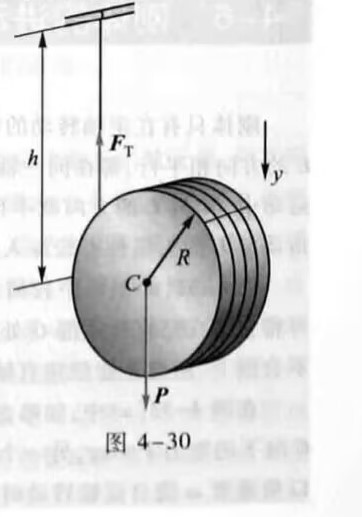
\includegraphics[width=0.5\textwidth]{img/4-30.jpg}
\end{figure}
如图,由此易知$a = \frac{P}{m_{eq}}$,即$a = \frac{2}{3}g $
\section{流体力学}
\subsection{伯努利方程}
$$  
    p + \frac{1}{2} \rho v^2 + \rho gh = C
$$
\subsection{泊肃叶方程}
对于在圆管中稳定流动的流体,有:
\begin{align*}
    Q_v &= \frac{\pi R^4 \Delta P}{8 \eta L} \\
    \bar{v} &= \frac{Q_v}{\pi R^2} = \frac{\Delta P R^2}{8 \eta L} \\
    w &= \frac{8\eta L}{R^2} \bar{v} = \Delta P
\end{align*}
$Q_v$为流体的流量,$\bar{v}$为流体的平均速度,$w$为损失的功率。
\subsection{斯托克斯公式}
对于一个小球在黏性流体中的运动,当小球的半径和速度均不大的时候有:
$$
    F = 6 \pi \eta r v 
$$
\section{第九章}
\subsection{单摆与复摆}
单摆的角频率和周期为:
\begin{align*}
    \omega &= \sqrt{\frac{g}{l}} \\
    T      &= 2\pi \sqrt{\frac{l}{g}}
\end{align*}
复摆的角频率和周期为:
\begin{align*}
    \omega &= \sqrt{\frac{mgl}{J}} \\
    T      &= 2\pi \sqrt{\frac{J}{mgl}}
\end{align*}
\subsection{两个同方向不同频率简谐振动的合成}
设现有两个简谐振动:
\begin{align*}
    x_1 &= A \cos(\omega_1 t ) \\
    x_2 &= A \cos(\omega_2 t )
\end{align*}
那么合成之后的振动方程为:
$$
    x = (2A \cos(\frac{\omega_2 - \omega_1}{2}t))\cos(\frac{\omega_2 + \omega_1}{2}t)
$$
由于我们认为$|\omega_1 + \omega_2| \gg |\omega_1 -\omega_2|$,
故我们将式子中的$|2A\cos(\frac{\omega_1 -\omega_2}{2})|$视为和振动的振幅。
而和振幅的频率为$\frac{|\omega_1-\omega_2|}{2\pi}$
\section{波动}
\subsection{波的传播速度}
理论和实验证明,在固体中,横波和纵波的传播速度为:
\begin{align*}
    v_{\text{横}} &= \sqrt{\frac{G}{\rho}} \\
    v_{\text{纵}} &= \sqrt{\frac{E}{\rho}}
\end{align*}
G、E分别为剪切模量和杨氏(弹性)模量,$\rho$为材料的密度。
在气体中,声速为:
$$
    v = \sqrt{\frac{K}{\rho}}
$$
\subsection{波的能量}
波的能量密度为:
$$
    w = \rho A^2 \omega^2 \sin^2 \omega\left(t - \frac{x}{u}\right)
$$
取一个周期的平均值,有:
$$
    \bar{w} = \frac{1}{2} \rho A^2 \omega^2
$$
平均能流为:
$$
    \bar{P} = \bar{w} u S
$$
而平均能流密度为:
$$
    I =\frac{\bar{P}}{S} = \bar{w}u = \frac{1}{2} \rho A^2 \omega^2 u
$$
\subsection{驻波}
驻波的波函数为:
$$
    y = 2A \cos 2\pi \frac{x}{\lambda} \cos 2\pi \nu t
$$
两个相邻的波节之间的距离为:
$$
    \Delta x = \frac{\lambda}{2}
$$
\subsection{多普勒效应}
当波源和观察者相对运动时,波的频率和波长会发生变化,这种现象被称为多普勒效应。
接受到的频率为:
$$
    \nu' = \frac{u \pm v_0}{u \mp v_s} \nu
$$
在上式中,$v_0$为波源的速度,$v_s$为观察者的速度,$u$为波的传播速度。
当观察者向波源靠近时,$v_0$取正号,否则取负号。
当波源向着观察者靠近时,$v_s$取负号,否则取正号。
\subsection{惠更斯原理}
惠更斯原理是波动光学的基础原理之一,
它的内容是:波的每一点都可以看作是次波源,次波源发出的波是原波的波前,波前是由无数个次波源发出的波构成的。
\begin{figure}[H]
    \centering
    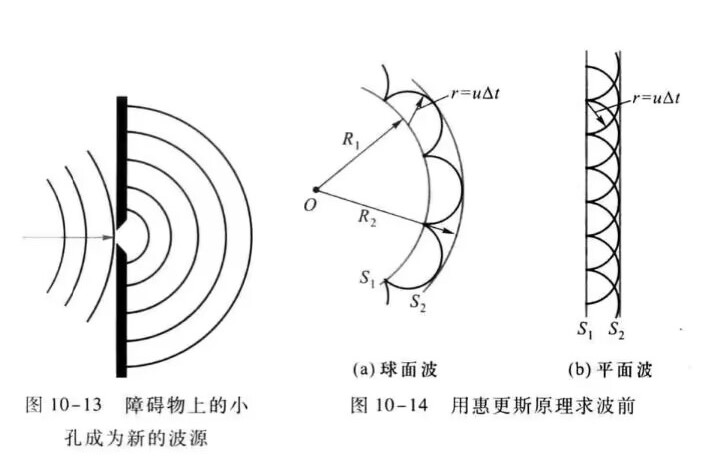
\includegraphics[width=0.7\textwidth]{img/10-13.jpg}
\end{figure}
\begin{figure}[H]
    \centering
    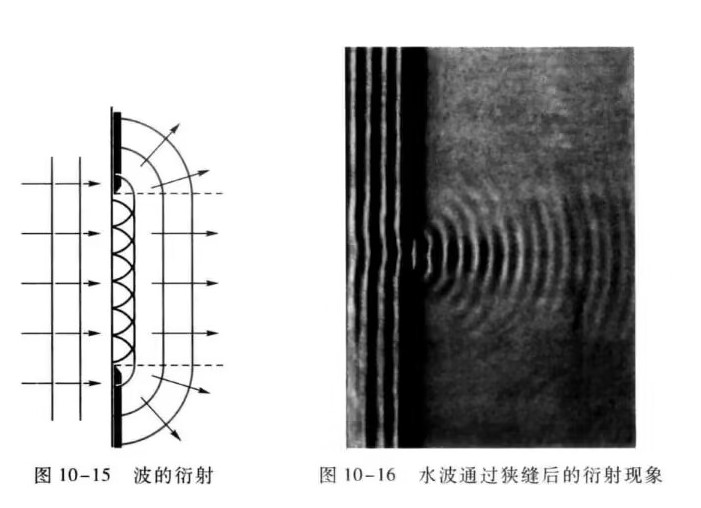
\includegraphics[width=0.7\textwidth]{img/10-15.jpg}
\end{figure}
\subsection{半波损失}
介质的密度$\rho$与波速$v$的乘积为波阻$Z$,即$Z = \rho v$。
$Z$大的称为波密介质,$Z$小的称为波疏介质。
当波从波疏介质传播到波密介质时,反射波的相位会发生$\pi$的跃变,这种现象被称为半波损失。
\section{相对论}
\subsection{洛伦兹变换}
洛伦兹变换为:
\begin{equation*}
    \begin{cases}
        x' = \frac{x - vt}{\sqrt{1 - \frac{v^2}{c^2}}} \\
        y' = y \\
        z' = z \\
        t' = \frac{t - \frac{v}{c^2}x}{\sqrt{1 - \frac{v^2}{c^2}}}
    \end{cases}
\end{equation*}
速度为:
\begin{equation*}
    \begin{cases}
        u_x' = \frac{u_x-v}{1-\frac{u_xv}{c^2}} \\
        u_y' = \frac{u_y}{\gamma(1-\frac{u_xv}{c^2})} \\
        u_z' = \frac{u_z}{\gamma(1-\frac{u_xv}{c^2})} \\
        \gamma = \frac{1}{\sqrt{1-\frac{v^2}{c^2}}}
    \end{cases}
\end{equation*}
洛伦兹变化的关键是认为光速是时空变换的特征向量,即光速不变。而伽利略变换的关键是一个同时性。
故于此相对的,洛伦兹变换有在一个参考系中同时发生的事,可能在另一个参考系中不同时发生。
\subsection{*时空矢量}
时空矢量$R$在一维的情况下可以表示为:
$$
    R = (ct,x)
$$
c为光速,t为时间,x为距离。
而时空矢量的长度为:
$$
    R^2 = c^2t^2 - x^2
$$
我们有以下的结论,在洛伦兹变换下,时空矢量的长度不变。
即:
\begin{align*}
    R^2 &= R'^2 \\
    c^2t^2 - x^2 &= c^2t'^2 - x'^2
\end{align*}
请自行用洛伦兹变换的结果验算。\\
其的理解是,在某一个$S$系中,我们有一个事件发生在$(ct,x)$处,而在另一个$S'$系中,我们有一个事件发生在$(ct',x')$处,那么这两个事件将满足上面的式子。
例题:
\begin{figure}[H]
    \centering
    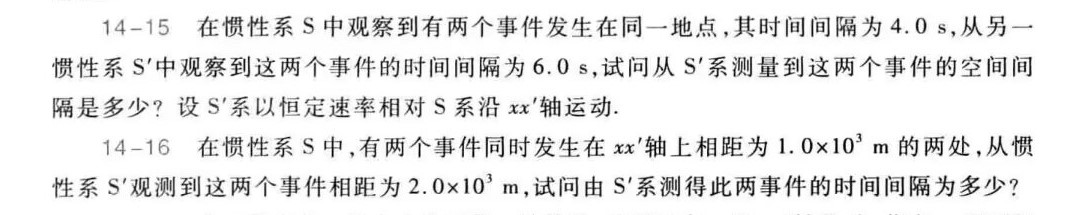
\includegraphics[width=0.9\textwidth]{img/14.jpg}
\end{figure}
我们都以其中一个事件作为坐标原点,那么有:
\begin{itemize}
    \item 14.15:
    \begin{align*}
        (ct)^2 - x^2 &= (ct')^2 - x'^2 \\
        (4c)^2 - 0 &= (6c)^2 - x'^2 \\
        x' &= \sqrt{20}c  \\
        &= 1.34 \times 10^9 m
    \end{align*}
    \item 14.16:
    \begin{align*}
        (ct)^2 - x^2 &= (ct')^2 - x'^2 \\
        0 - (1\times 10^3)^2 &= (t')^2 - (2 \times 10^3)^2 \\
        t' &= \sqrt{\frac{3\times 10^6}{9\times 10^{16}}} \\
        &= 5.77 \times 10^{-6}s
    \end{align*}
\end{itemize}
\subsection{相对论的时空观}
在相对论中,我们有三个效应,即:
\begin{itemize}
    \item 尺缩效应
    \item 钟慢效应
    \item 增重效应
\end{itemize}
只需要知道,上面的三个效应的放缩比都为$\gamma$即可。
(原长最长,原时最短,\sout{原神启动},原重最轻)
\subsection{光的多普勒效应}
光的多普勒效应为:
$$
    \frac{\nu_a}{\nu_b} = \sqrt{\frac{1-\beta}{1+\beta}}(\text{B离A而去})
$$
$\beta=\frac{v}{c}$,$v$为观察者相对光源的速度。
同理,相靠近的话,$\beta$取负号。
\subsection{相对论的动量与能量}
相对论中的动量和动能有以下的关系:
\begin{align*}
    (pc)^2 +E_0^2 &= E^2 \\
    E_k &= E - E_0
\end{align*}
光子的动量为:
$$
    p = \frac{h}{\lambda}
$$
\section{静电场}
\subsection{电偶极子}
电偶极子是指由两个等量异号的电荷组成的系统。\\
我们有以下的结论:\\
由电偶极子组成的系统的电势为:
$$
    V = \frac{1}{4\pi \varepsilon_0} \frac{p \cos \theta}{r^2}
$$
而任意处的电场为:
$$
    \vec{E} = (\frac{1}{4\pi \varepsilon_0} \frac{p(1-3\cos^2\theta)}{r^3},\frac{1}{4\pi \varepsilon_0} \frac{3p\sin\theta\cos\theta}{r^3})
$$
\begin{figure}[H]
    \centering
    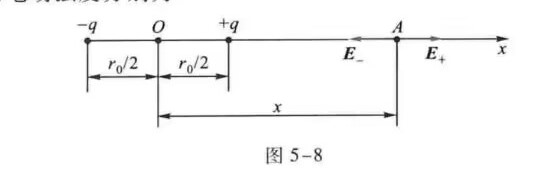
\includegraphics[width=0.5\textwidth]{img/5-8.jpg}
\end{figure}
\begin{figure}[H]
    \centering
    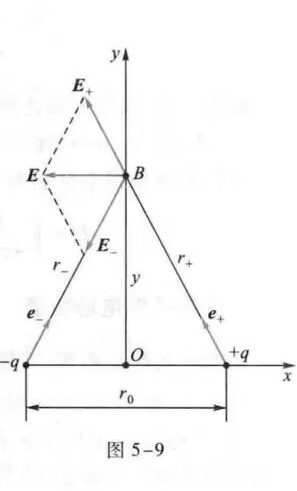
\includegraphics[width=0.4\textwidth]{img/5-9.jpg}
\end{figure}
由此便非常易得图5-8和5-9的结果,带入即可。
\begin{align*}
    \vec{E_{5-8}} &= (-\frac{1}{4\pi \varepsilon_0} \frac{2p}{r^3},0) \\
    \vec{E_{5-9}} &= (-\frac{1}{4\pi \varepsilon_0} \frac{p}{r^3},0)
\end{align*}
% *证明:\\
% 我们先求出势函数,再求出电场强度。\\
% 令$r$为点$P$到$O$的距离,$\theta$为$OP$与$x$轴的夹角,那么有:
% \begin{align*}
%     u &= \frac{1}{4\pi \varepsilon_0} \left( \frac{q}{\sqrt{r^2+\left(\frac{r_0}{2}\right)^2 - r r_0 \cos\theta}} - \frac{q}{\sqrt{r^2+\left(\frac{r_0}{2}\right)^2 + r r_0 \cos\theta}}\right) \\
%     &= \frac{1}{4\pi \varepsilon_0} \frac{q}{r} \frac{\sqrt{1+\left(\frac{r_0}{2r}\right)^2 + r_0 \cos\theta} - \sqrt{1+\left(\frac{r_0}{2r}\right)^2 -  r_0 \cos\theta}}{\sqrt{\left(1+\left(\frac{r_0}{2r}\right)^2\right)^2 - \left(r_0 \cos\theta\right)^2}}\\
%     when: \lim_{\frac{r_0}{r} \to 0} : \\ 
%     &= \frac{1}{4\pi \varepsilon_0} \frac{qr_0\cos \theta}{r^2} \\
%     &= \frac{1}{4\pi \varepsilon_0} \frac{p \cos \theta}{r^2}
% \end{align*}
% \footnote{上面分子用二项式展开,忽略高阶无穷小即可得到该结果}
% 下面推导电场强度:
% \begin{align*}
%     \frac{\partial u}{\partial r} &= -\frac{1}{4\pi \varepsilon_0} \frac{2 p \cos \theta}{r^3} \\
%     \frac{\partial u}{\partial \theta} &= -\frac{1}{4 \pi \varepsilon_0} \frac{p \sin \theta}{r^2} \\
%     \frac{\partial u}{\partial x} &= \frac{\partial u}{\partial (r,\theta)} \frac{\partial (r,\theta)}{\partial x} \\
%     &= -\frac{1}{4\pi \varepsilon_0} \frac{2 p \cos\theta}{r^3} \cdot \cos\theta - \frac{1}{4\pi \varepsilon_0} \frac{p \sin\theta}{r^2} \cdot -\frac{ \sin\theta}{r} \\
%     &= \frac{1}{4\pi \varepsilon_0} \frac{p(1-3\cos^2\theta)}{r^3} = -E_x \\
%     \frac{\partial u}{\partial y} &= \frac{\partial u}{\partial (r,\theta)} \frac{\partial (r,\theta)}{\partial y} \\
%     &= -\frac{1}{4\pi \varepsilon_0} \frac{2 p \cos\theta}{r^3} \cdot \sin\theta - \frac{1}{4\pi \varepsilon_0} \frac{p \sin\theta}{r^2} \cdot \frac{ \cos\theta}{r} \\
%     &= -\frac{1}{4\pi \varepsilon_0} \frac{3p\sin\theta\cos\theta}{r^3} =-E_y
% \end{align*}
\subsection{几种常见的电场,电势分布}
\begin{itemize}
    \item 带电圆环:
    \begin{figure}[H]
        \centering
        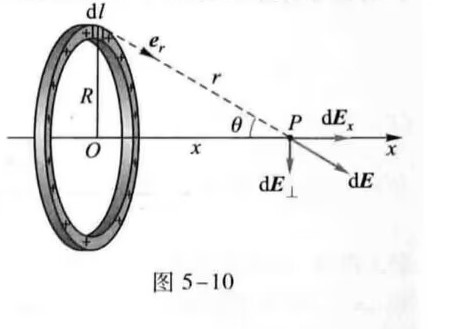
\includegraphics[width=0.4\textwidth]{img/5-10.jpg}
    \end{figure}
    \begin{align*}
        E &= \frac{1}{4\pi \varepsilon_0} \frac{qx}{(x^2 + R^2)^{3/2}}\\
        V &= \frac{1}{4\pi \varepsilon_0} \frac{q}{\sqrt{x^2 + R^2}}
    \end{align*}
    
    \item 带电圆盘:
    \begin{figure}[H]
        \centering
        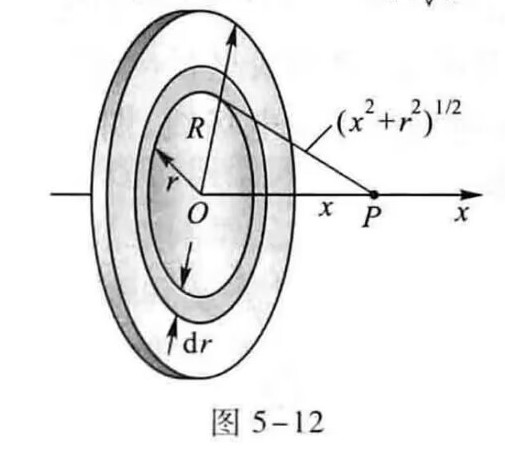
\includegraphics[width=0.4\textwidth]{img/5-12.jpg}
    \end{figure}
    \begin{align*}
        E &= \frac{\sigma }{2 \varepsilon_0} \left(1-\frac{x}{\sqrt{x^2 + R^2}}\right) \\
        V &= \frac{\sigma}{2\varepsilon_0} (\sqrt{x^2+R^2} - x)
    \end{align*}
    \item 无限长带电直线:
    \begin{figure}[H]
        \centering
        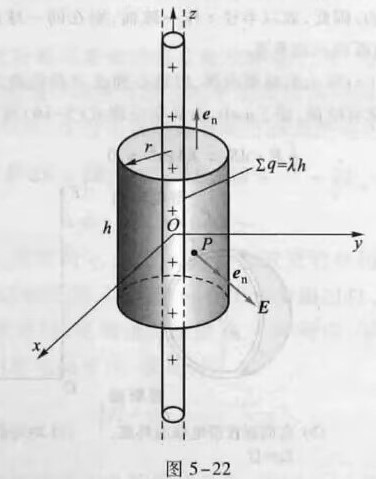
\includegraphics[width=0.4\textwidth]{img/5-22.jpg}
    \end{figure}
    $$
        E = \frac{\lambda}{2\pi \varepsilon_0 r}
    $$
    \item 无限大均匀带电平面:
    \begin{figure}[H]
        \centering
        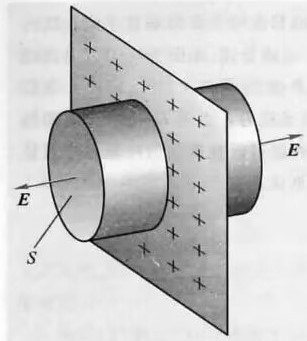
\includegraphics[width=0.4\textwidth]{img/5-23.jpg}
    \end{figure}
    $$
        E = \frac{\sigma}{2\varepsilon_0}
    $$
    即对应的带电圆盘当$R \to \infty$时的情况。
    \item 带电圆弧:
    \begin{figure}[H]
        \centering
        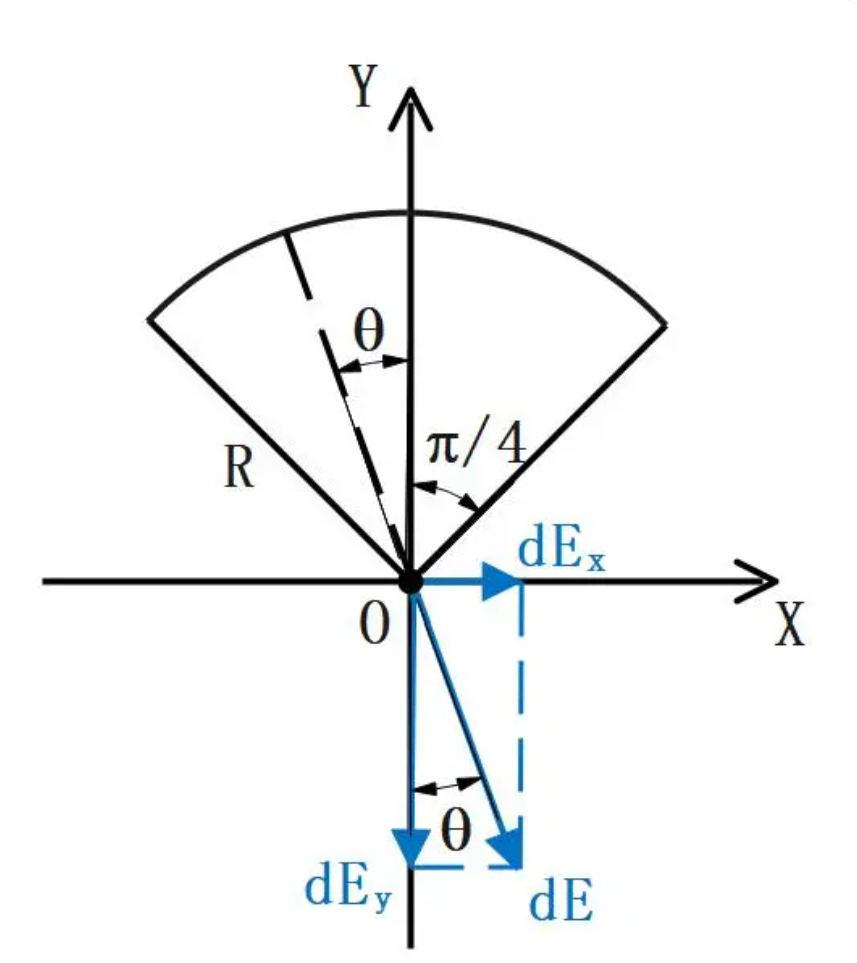
\includegraphics[width=0.4\textwidth]{img/rho.png}
    \end{figure}
    圆心处的电场强度方向延圆弧的角平分线方向
    \begin{align*}
        E &= \frac{1}{2\pi \varepsilon_0} \frac{\lambda}{R} \sin \frac{\theta}{2} \\
        V &= \frac{1}{4\pi\varepsilon_0} \lambda \theta
    \end{align*}
    \item 带电直线:
    \begin{figure}[H]
        \centering
        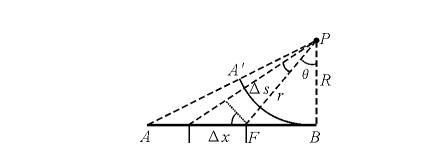
\includegraphics[width=0.6\textwidth]{img/linerho.png}
    \end{figure}
    对于带电直线,我们有以下的结论:\\
    如图,其的电场强度可以被等效为一段带电圆弧产生的电场强度。
    % \begin{align*}
    %     x &= R \tan \theta \\
    %     \Delta x &= R \frac{1}{\cos^2 \theta} \Delta \theta \\
    %     \text{对于直线上的$\Delta x$产生的电场强度为:} \\
    %     \Delta E &= \frac{1}{2\pi \varepsilon_0} \frac{\lambda \Delta x}{(\frac{R}{\cos\theta})^2} \cos\theta \\
    %     & = \frac{1}{2\pi \varepsilon_0} \frac{\lambda \Delta x}{R^2} \cos\theta \\
    %     \text{对于对应圆弧的电场强度有:} \\
    %     \Delta E &= \frac{1}{2\pi \varepsilon_0} \frac{\lambda \Delta x}{R^2} \cos\theta \\
    %     \text{那么显然成立}
    % \end{align*}
    \footnote{请注意电势是不等效的!对于二维的情况,即带电圆盘,电场强度也不等效} \\
    那么,就不难求出一般情况下的电场强度。特别的,当其在延长线上时,电场强度为:
    $$
        E = \frac{1}{\pi \varepsilon_0} \frac{Q}{4r^2 - L^2}
    $$
    当其在中垂线上时,电场强度为:
    $$
        E = \frac{1}{2\pi \varepsilon_0} \frac{Q}{r\sqrt{4r^2 + L^2}}
    $$
    可自行验证在中垂线上的情景是符合对应的圆弧的电场强度的。\\
    再特别的,当直线为无限长时,即$\lim_{\theta \to \pi}$时,有:
    $$
        E = \frac{1}{2\pi \varepsilon_0} \frac{\lambda}{r}
    $$
    \item 带电球体:
    \begin{figure}[H]
        \centering
        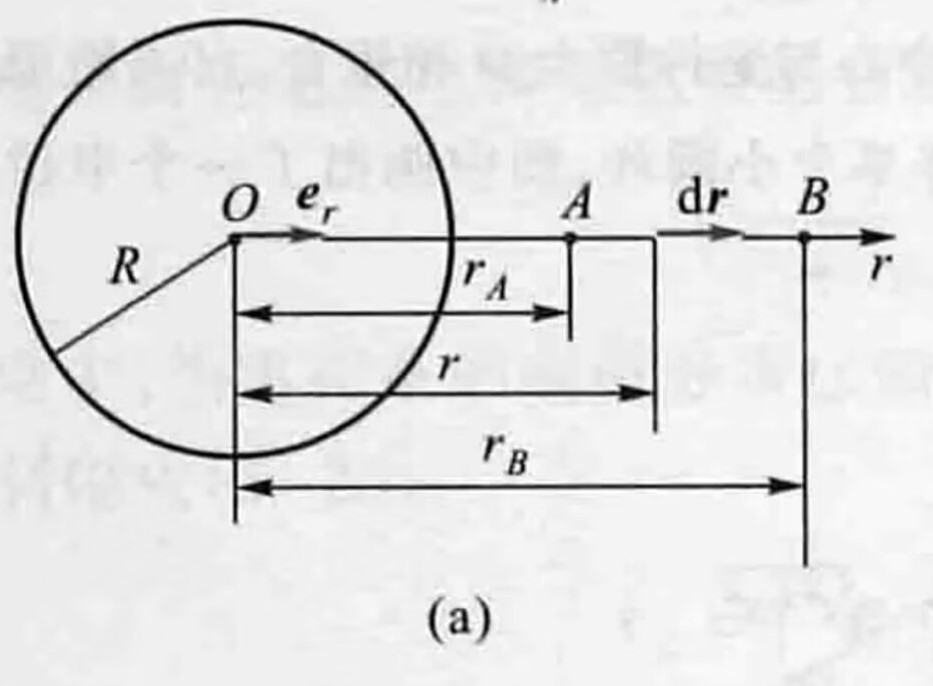
\includegraphics[width=0.4\textwidth]{img/5-31.jpg}
    \end{figure}
    \begin{equation*}
        \begin{cases}
            E = \frac{1}{4\pi \varepsilon_0} \frac{4 \rho r}{3} & r < R \\
            E = \frac{1}{4\pi \varepsilon_0} \frac{4 \rho R^3}{3r^2} & r > R
        \end{cases}
    \end{equation*}
    \begin{equation*}
        \begin{cases}
            V = \frac{1}{4\pi \varepsilon_0} \frac{4 \rho r^2}{3} & r < R \\
            V = \frac{1}{4\pi \varepsilon_0} \frac{4 \rho R^3}{3r} & r > R
        \end{cases}
    \end{equation*}
\end{itemize}
\subsection{高斯定理}
高斯定理为:
$$
    \ooint \vec{E} \cdot d\vec{S} = \frac{Q_{\text{enc}}}{\varepsilon_0}
$$
其中$Q_{\text{enc}}$为闭合曲面内的净电荷量。
\subsection{电场力的相似三角形}
众所周知,高中如果在分析受力平衡的时候,如果采用相似三角形的方法,那么这个题里面的力要么是恒定的、方向不变的、或与距离成正比的。\\
电场一般很难满足这些条件,但也有特殊情况。
\begin{figure}[H]
    \centering
    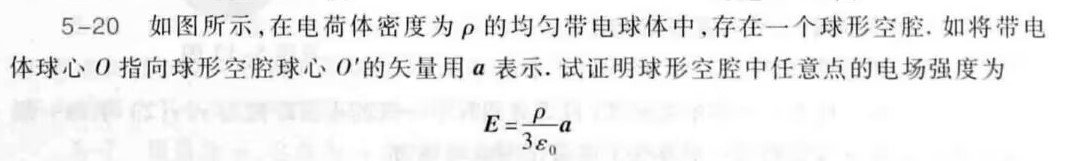
\includegraphics[width=1\textwidth]{img/x5-20.jpg}
\end{figure}
我们可以认为球形空腔是由于此处存在负的$\rho$ ,那么易知,两种电荷的电场力是能够构造相似三角形的,即与距离成正比。\\
那么不难求得5-20和5-21的结果,请自行练手计算。
\section{静电场中的导体与介质}
\subsection{导体的静电平衡}
导体的静电平衡有以下的特点:
\begin{itemize}
    \item 导体内部的电场为0
    \item 导体表面的电场垂直于表面
    \item 导体的电荷分布只可能分布在内表面或外表面
\end{itemize}
静电平衡的两种应用:
\begin{itemize}
    \item 用空腔导体屏蔽外电场
    \item 用接地空腔导体屏蔽内电场
    \begin{figure}[H]
        \centering
        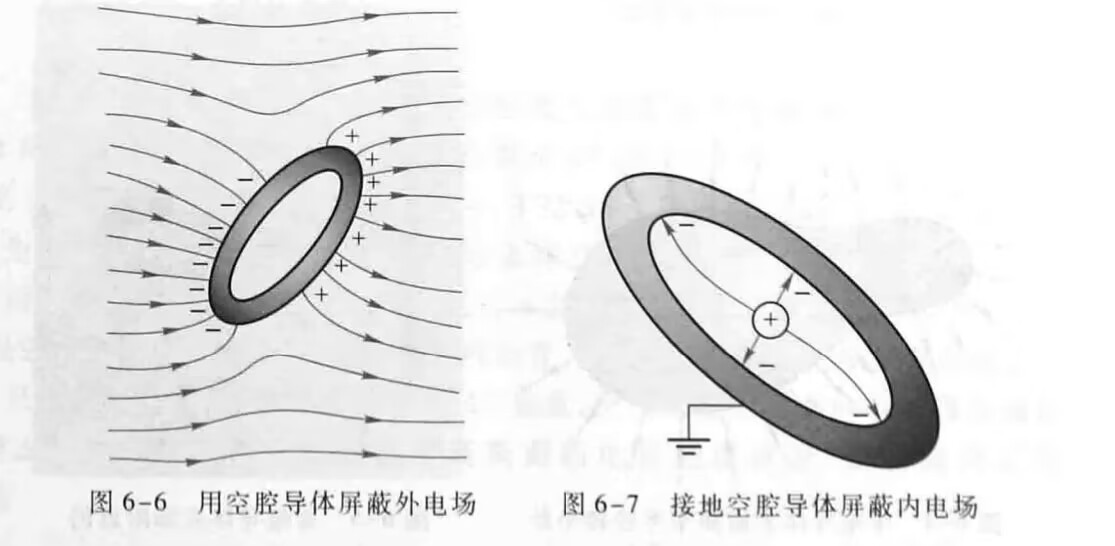
\includegraphics[width=0.5\textwidth]{img/6-6.jpg}
    \end{figure}
\end{itemize}
\subsection{电位移,极化强度,极化电荷}
\begin{figure}[H]
    \centering
    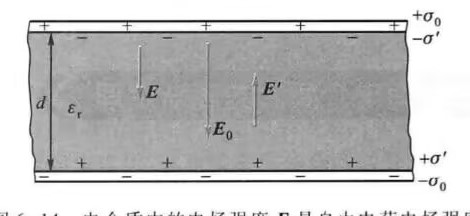
\includegraphics[width=0.5\textwidth]{img/6-14.jpg}
\end{figure}
有:
\begin{align*}
    \vec{E'} &= \frac{\varepsilon_r -1}{\varepsilon_r} \vec{E_0} \\
    \sigma' &= \frac{\varepsilon_r -1}{\varepsilon_r} \sigma_0 \\
    \vec{P} &= (\varepsilon_r -1) \varepsilon_0 \vec{E_0} = \varepsilon_0 \chi_e \vec{E_0} \\
    \vec{D} &= \varepsilon_0 \vec{E} + \vec{P} \\
    \vec{D} &= \varepsilon \vec{E} = \varepsilon_0 \varepsilon_r \vec{E}
\end{align*}
\footnote{请自行对照书本死记硬背}
在电介质中,高斯定理为:
$$
    \ooint \vec{D} \cdot d\vec{S} = Q_{\text{enc}}
$$
\subsection{各种电容器的电容}
\begin{itemize}
    \item 平行板电容器:
    \begin{figure}[H]
        \centering
        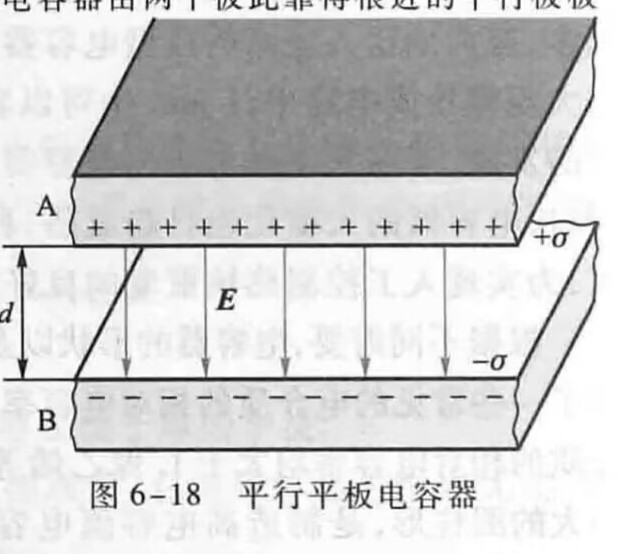
\includegraphics[width=0.5\textwidth]{img/6-18.jpg}
    \end{figure}
    $$
        C = \varepsilon \frac{S}{d}
    $$
    \item 球形电容器:
    \begin{figure}[H]
        \centering
        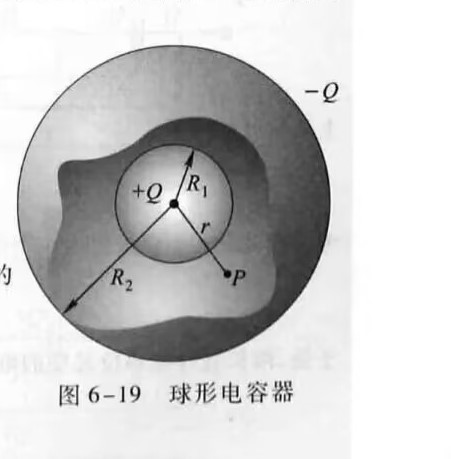
\includegraphics[width=0.5\textwidth]{img/6-19.jpg}
    \end{figure}
    $$
        C = 4\pi \varepsilon \frac{R_1R_2}{R_2 - R_1}
    $$
    特别的,当$R_2 \to \infty$时,有:
    $$
        C = 4\pi \varepsilon R_1
    $$
    即孤立球形导体的电容。
    \item 长直导线:
    \begin{figure}[H]
        \centering
        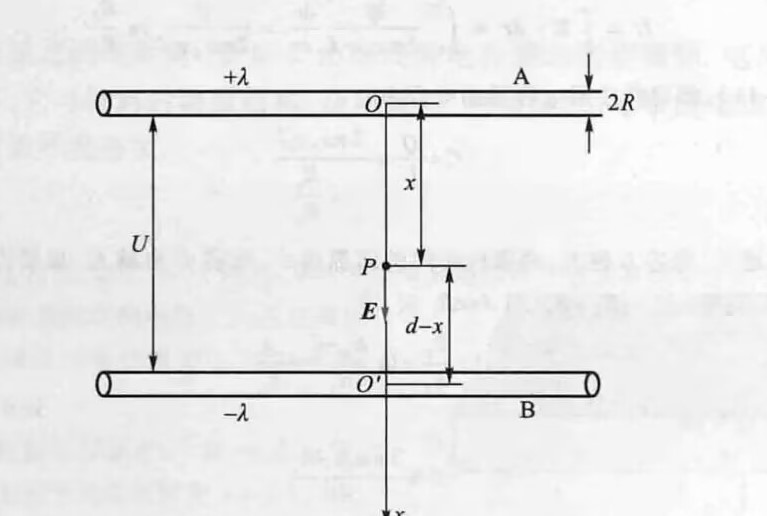
\includegraphics[width=0.5\textwidth]{img/6-20.jpg}
    \end{figure}
    单位长度的电容为:
    $$
        C \approx \frac{\pi \varepsilon}{\ln \frac{d}{R}}
    $$
    \item 圆柱形电容器:
    \begin{figure}[H]
        \centering
        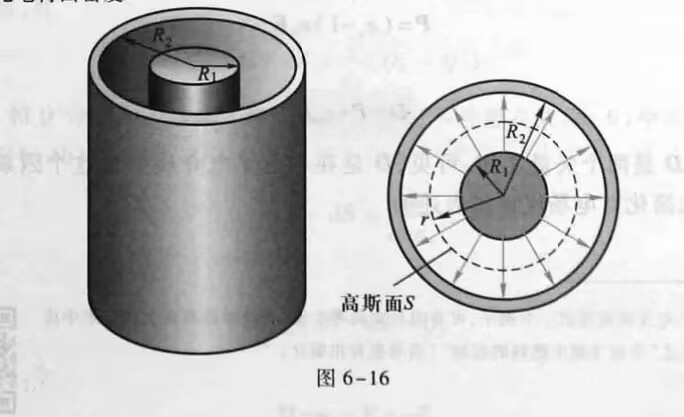
\includegraphics[width=0.4\textwidth]{img/6-16.jpg}
    \end{figure}
    $$
        C = 2\pi \varepsilon \frac{L}{\ln \frac{R_2}{R_1}}
    $$
    当两极板之间的间隙极小,即$R_2 \to R_1$时,有:
    $$
        C \approx \varepsilon \frac{S}{d}
    $$
    即认为其是平行板电容器。
\end{itemize}
\subsection{电容的串并联}
\begin{itemize}
    \item 串联:
    $$
        \frac{1}{C} = \frac{1}{C_1} + \frac{1}{C_2} + \cdots
    $$
    \item 并联:
    $$
        C = C_1 + C_2 + \cdots
    $$
\end{itemize}
\subsection{电容器的能量}
电容器的能量为:
$$
    W = \frac{1}{2} CU^2 = \frac{1}{2} QU
$$
而单位体积中的能量密度为:
$$
    w = \frac{1}{2} \varepsilon E^2
$$
故电容器的能量为:
$$
    W = \iiint w dV
$$
\subsection{*电容器的冲放电}
电容的充电过程为:
$$
    U = U_0 (1 - e^{-\frac{t}{RC}})
$$
电容的放电过程为:
$$
    U = U_0 e^{-\frac{t}{RC}}
$$
其中,$RC$为电容器的时间常数$\tau$。
\section{第七章}
\subsection{电流密度}
由微观有:
$$
    I = \iint \vec{j} \cdot d\vec{S}
$$
则有:
\begin{align*}
    I = neSv \\
    j = env
\end{align*}
\subsection{欧姆定律微分形式}
欧姆定律微分形式为:
$$
    \vec{j} = \sigma \vec{E}
$$
$\sigma$为电导率。
\subsection{比奥-萨伐尔定律}
比奥-萨伐尔定律为:
$$
    d\vec{B} = \frac{\mu_0}{4\pi} \frac{Id\vec{l}\sin\theta}{r^2}
$$
\subsection{各种常见的磁场分布}
\begin{itemize}
    \item 直导线
    \begin{figure}[H]
        \centering
        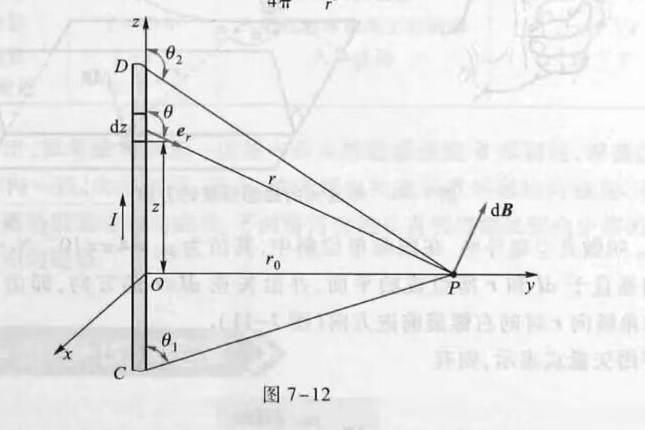
\includegraphics[width=0.5\textwidth]{img/7-12.jpg}
    \end{figure}
    $$
        B = \frac{\mu_0I}{4\pi r_0} (\cos \theta_1 - \cos \theta_2)
    $$
    \item 圆环
    \begin{figure}[H]
        \centering
        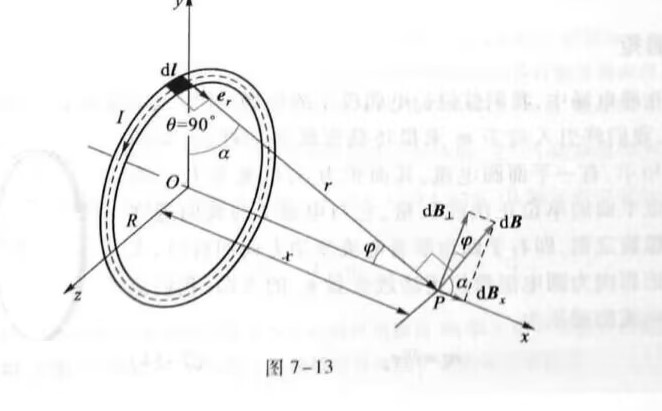
\includegraphics[width=0.5\textwidth]{img/7-13.jpg}
    \end{figure}
    $$
        B = \frac{\mu_0I}{2} \frac{R^2}{(R^2 + x^2)^{3/2}}
    $$
    当 $x = 0$时,有:
    $$
        B = \frac{\mu_0I}{2R}
    $$
    特别的,当$x \gg R$时,有:
    $$
        B = \frac{\mu_0I}{2} \frac{R^2}{x^3}
    $$
    亦可写成磁矩形式:
    $$
        \vec{B} = \frac{\mu_0}{2\pi} \frac{\vec{m} }{x^3}
    $$
    \item 密绕螺线管
    \begin{figure}[H]
        \centering
        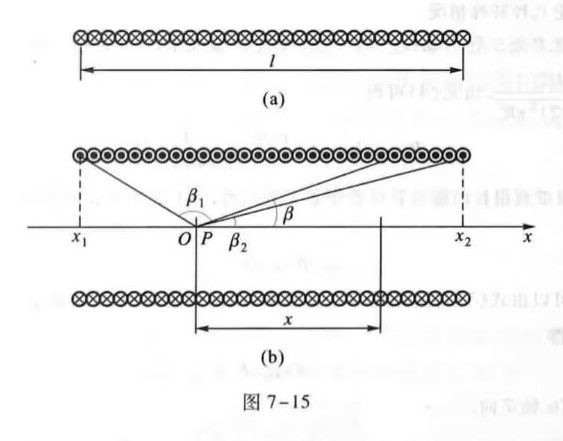
\includegraphics[width=0.5\textwidth]{img/7-15.jpg}
    \end{figure}
    $$
        B = \frac{\mu_0 nI}{2} (\cos \beta_2 - \cos \beta_1)
    $$
    当认为螺线管是无限长时,有:
    $$
        B = \mu_0 n I
    $$
    而在其的一端,有:
    $$
        B = \frac{\mu_0 n I}{2} 
    $$
    \item 旋转圆盘
    \begin{figure}[H]
        \centering
        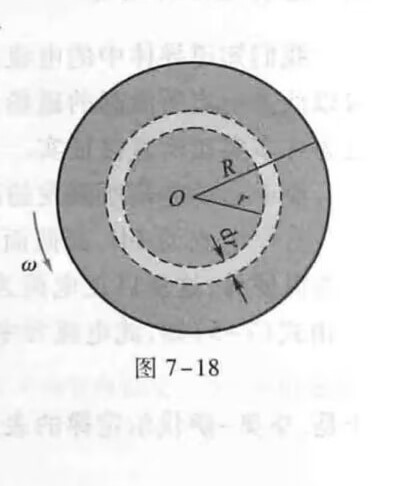
\includegraphics[width=0.5\textwidth]{img/7-18.jpg}
    \end{figure}
    $$
        B = \frac{\mu_0 \omega \sigma R}{2}
    $$
    \item 无限长直导线
    \begin{figure}[H]
        \centering
        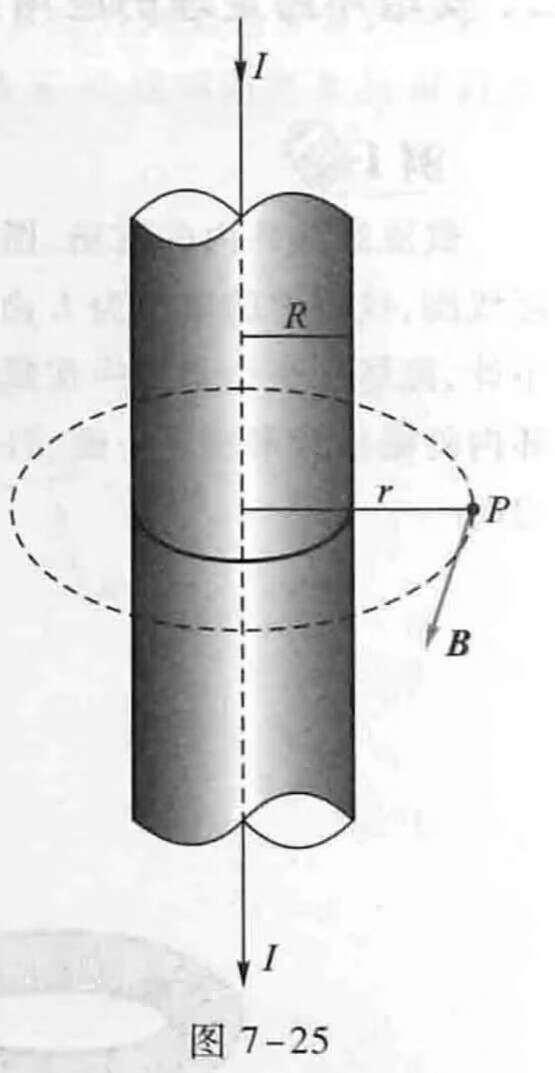
\includegraphics[width=0.4\textwidth]{img/7-25.jpg}
    \end{figure}
    在其内部,有:
    $$
        B = \frac{\mu_0 Ir}{2\pi R^2} (r<R)
    $$
    \item 圆形密绕线圈
    \begin{figure}[H]
        \centering
        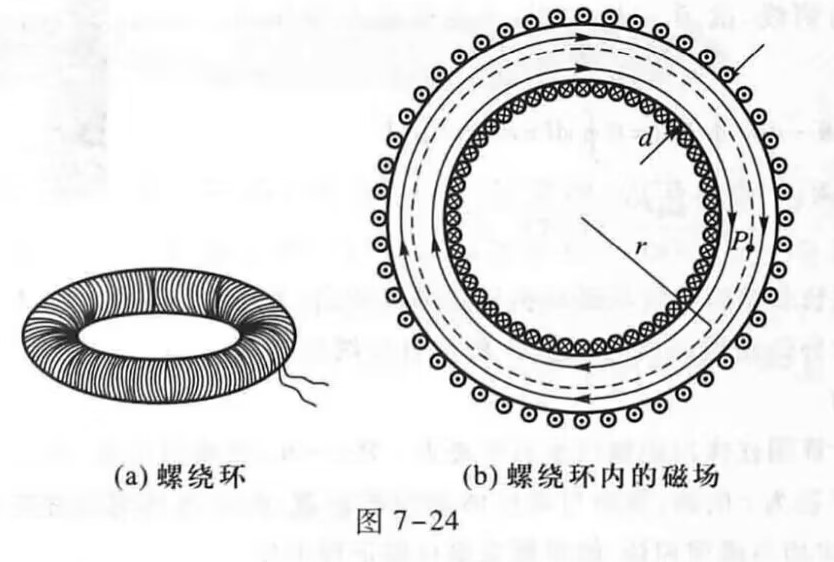
\includegraphics[width=0.7\textwidth]{img/7-24.jpg}
    \end{figure}
    $$
        B = \frac{\mu_0 N I}{2\pi r}
    $$
    对于圆环中心轴线上的磁场,有:
    $$
        B = \mu_0 n I
    $$
\end{itemize}
\subsection{磁场的高斯定理}
磁场的高斯定理为:
$$
    \ooint \vec{B} \cdot d\vec{S} = 0
$$
\subsection{安培环路定理}
安培环路定理为:
$$
    \oint \vec{B} \cdot d\vec{l} = \mu_0 I_{\text{enc}}
$$
\subsection{带电粒子在磁场中的运动}
带电粒子在电磁场中的运动有以下的特点:
$$
    F = q\vec{v} \times \vec{B} + q \vec{E}
$$
\begin{itemize}
    \item 粒子的轨道是一个圆
    \item 粒子的轨道半径为:
    $$
        r = \frac{mv}{qB}
    $$
    \item 粒子的周期为:
    $$
        T = \frac{2\pi m}{qB}
    $$
    \item 粒子的角频率为:
    $$
        \omega = \frac{qB}{m}
    $$
    \item 磁场力\sout{never gonna you up}不做功
    \item 以及请自行回忆起高中的正则动量的知识or配速法or大学的解微分方程的知识 以防考察带电粒子在速度选择器中的运动
\end{itemize}
\subsection{霍尔效应}
\begin{figure}[H]
    \centering
    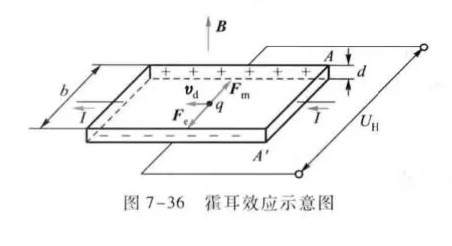
\includegraphics[width=0.5\textwidth]{img/7-36.jpg}
\end{figure}
霍尔电压为:
$$
    U_H = \frac{IB}{nqd}
$$
霍尔系数为:
$$
    R_H = \frac{1}{nq}
$$
\subsection{载流导线在磁场中的受力}
载流导线在磁场中的受力为:
$$
    d\vec{F} = I d\vec{l} \times \vec{B}
$$
\begin{figure}[H]
    \centering
    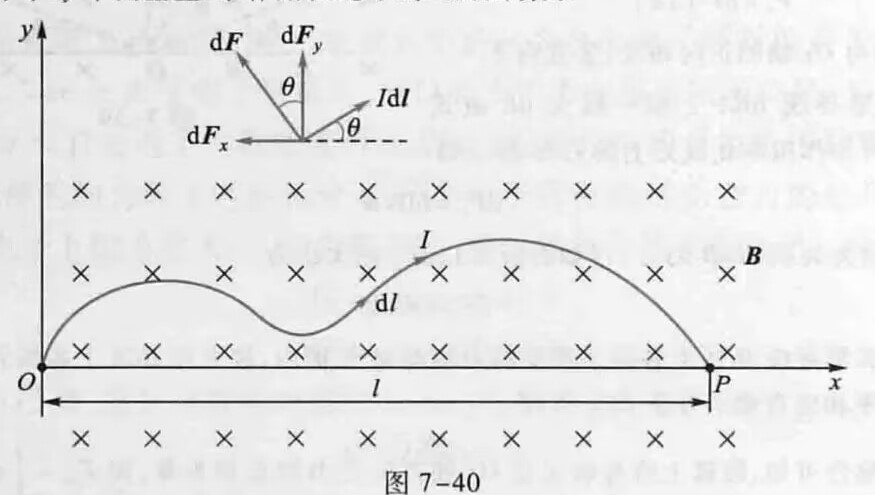
\includegraphics[width=0.5\textwidth]{img/7-40.jpg}
\end{figure}
对于在磁场中的闭合线圈,有:
$$
    \vec{F}_{\text{合}} = 0
$$
故对于这种不规则的导线,我们可以选择一条更合适的路径来计算。
\subsection{线圈的磁力矩}
\begin{figure}[H]
    \centering
    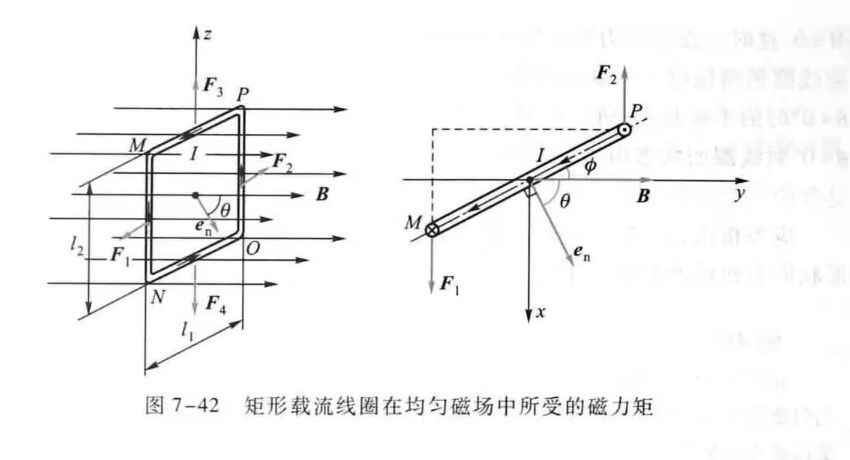
\includegraphics[width=0.7\textwidth]{img/7-42.jpg}
\end{figure}
线圈的磁力矩为:
$$
    \vec{M} =NIS\vec{e_n}\times \vec{B}=N \vec{m} \times \vec{B}
$$
\subsection{磁介质}
磁介质表面的磁化电流面密度为:
$$
    I_s = M
$$
$M$为磁化强度。
磁场强度为:
$$
    \vec{H} = \frac{\vec{B}}{\mu_0} - \vec{M}
$$
在线性磁介质中,有:
$$
    M = \chi_m H
$$
$\chi_m$为磁化率。
称$1+\chi_m$为相对磁导率。
则有:
$$
    \vec{B} = \mu_0\mu_r \vec{H} = \mu \vec{H}
$$
那么安培环路定理为:
$$
    \oint \vec{H} \cdot d\vec{l} = I_{\text{enc}}
$$
\section{第八章}
\subsection{电磁感应定律}
电磁感应定律为:
$$
    \varepsilon = -\frac{d\Phi}{dt}
$$
\subsection{动生电动势}
动生电动势为:
$$
    \varepsilon = vBl
$$
方向可以用右手定则来判断。\\
例如圆盘发电机,有:
\begin{figure}[H]
    \centering
    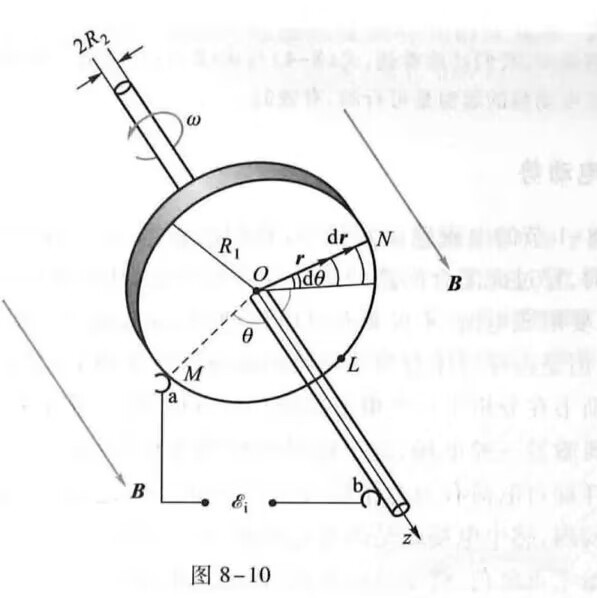
\includegraphics[width=0.5\textwidth]{img/8-10.jpg}
\end{figure}
$$
    U = \frac{1}{2} B (R_1^2 - R_2^2) \omega
$$
高中学过的线圈发电机,有:
$$
    U = NBS\omega
$$
\subsection{感生电动势}
感生电动势用$E_k$表示,有:
$$
    \oint \vec{E}_k \cdot d\vec{l} = -\frac{d\Phi}{dt}
$$
\subsection{自感与互感}
穿过回路的磁通量与电流成正比,称为自感。
$$
    \varPhi = LI
$$
长直螺线管的自感为:
$$
    L = \mu n^2 V
$$
互感即一个线圈的电流激发的磁场对另一个线圈产生的感应电动势。
\begin{align*}
    \varPhi_{21} &= M_{21}I_1 \\
    \varPhi_{12} &= M_{12}I_2 \\
    M_{21} &= M_{12}
\end{align*}
注意,一般而言,计算互感和自感系数的时候,都是用$L = \frac{\varPsi}{I}$ 计算的,而$\varPsi = N \Phi$ 称为磁链。
注意,这里的$N$是指线圈的匝数。对于一些特殊的线圈,$N$不一定是整数,例如对于后面的一对导线的内自感的计算,其的$N=0.5$,
故更加推荐用计算磁场能量的方法来计算自感和互感。
\subsection{电磁场的能量}
磁场的能量可以表示为:
$$
    W = \frac{1}{2} LI^2
$$
磁场的能量密度为:
$$
    w_m =  \frac{1}{2\mu} B^2 = \frac{1}{2}\mu H^2 = \frac{1}{2} BH
$$
\subsection{一些的自感}
\begin{itemize}
    \item 同轴电缆
    \begin{figure}[H]
        \centering
        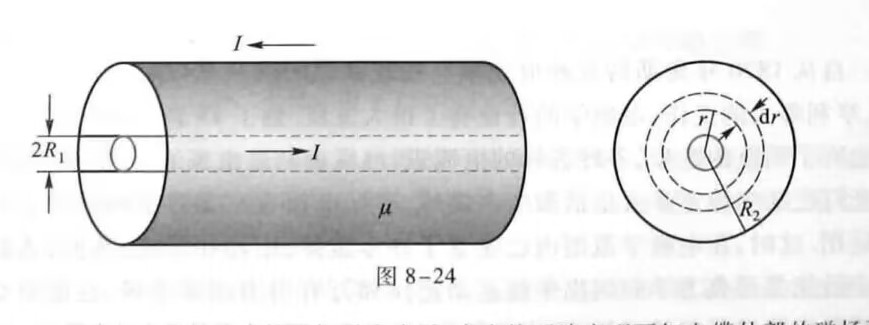
\includegraphics[width=0.5\textwidth]{img/8-24.jpg}
    \end{figure}
    $$
        L = \frac{\mu}{2\pi} \ln \frac{R_2}{R_1}
    $$
    \item 一对导线
    \begin{figure}[H]
        \centering
        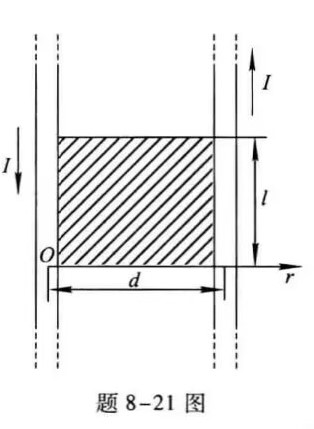
\includegraphics[width=0.5\textwidth]{img/8-21.jpg}
    \end{figure}
    其的自感$L = L_1 +2L_2$,$L_1$称为内自感,$L_2$称为外自感。
    \begin{align*}
        L_1 &= \frac{\mu_0l}{\pi} ln \frac{d-a}{a} \\
        L_2 &= \frac{\mu_0 l}{8\pi}
    \end{align*}
\end{itemize}
\subsection{位移电流}
电位移通量为:
$$
    \varPsi = SD
$$
位移电流为:
$$
    I_d = \frac{d\varPsi}{dt}
$$
位移电流密度为:
$$
    \vec{j}_d =  \frac{\partial \vec{D}}{\partial t}
$$
故将安培环路定理改为:
$$
    \oint \vec{H} \cdot d\vec{l} = I_{\text{enc}} + I_d = \int (\vec{j}_c + \frac{\partial D}{\partial t} )\cdot d\vec{S}
$$
麦克斯韦方程组为:
\begin{equation*}
    \begin{cases}
        \nabla \times \vec{E} = -\frac{\partial \vec{B}}{\partial t} \\
        \nabla \times \vec{H} = \vec{j}_c + \frac{\partial \vec{D}}{\partial t} \\
        \nabla \cdot \vec{D} = \rho \\
        \nabla \cdot \vec{B} = 0
    \end{cases}
\end{equation*}
积分形式为:
\begin{align*}
    \oint \vec{E} \cdot d\vec{l} &=  \iint -\frac{d \vec{B}}{dt}  \cdot d\vec{S} \\
    \oint \vec{H} \cdot d\vec{l} &= \iint (\vec{j}_c  + \frac{\partial \vec{D}}{\partial t}) d\vec{S} \\
    \ooint \vec{D} \cdot d\vec{S} &= Q_{\text{enc}} \\
    \ooint \vec{B} \cdot d\vec{S} &= 0
\end{align*}
\begin{figure}[H]
    \centering
    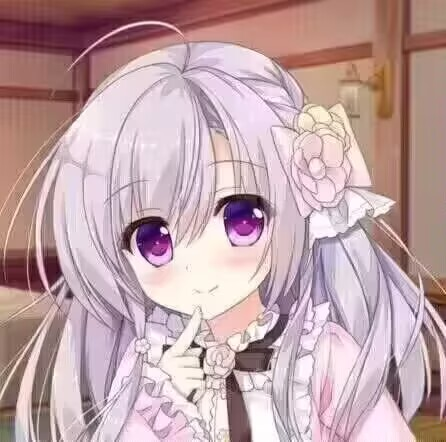
\includegraphics[width=0.5\textwidth]{img/source.jpg}
    \caption{事已至此,先吃饭吧}
\end{figure}
\end{document}